\documentclass[answers]{exam}

\usepackage{amsmath}
\usepackage{amssymb}
\usepackage{geometry}
\usepackage{venndiagram}
\usepackage{graphics}
\usepackage{graphicx}
\usepackage{tikz}
\usepackage{listings}
\usepackage{hyperref}
\usepackage{float}

\lstset{
    basicstyle=\ttfamily,
    columns=fullflexible,
    frame=single,
    breaklines=true,
    postbreak=\mbox{\textcolor{red}{$\hookrightarrow$}\space},
}

\geometry{
    bottom=2cm, % Adjust this value as needed to leave space for the answer boxes
}

% Header and footer.
\pagestyle{headandfoot}
\runningheadrule
\runningfootrule
\runningheader{EE/CE 468/468 Mobile Robotics}{Homework 4}{Fall 2023}
\runningfooter{}{Page \thepage\ of \numpages}{}
\firstpageheader{}{}{}

\boxedpoints
\printanswers

\newcommand{\uvec}[1]{\boldsymbol{\hat{\textbf{#1}}}}
\newcommand\union\cup
\newcommand\inter\cap
\newcommand\ul\underline
\newcommand\ol\overline

\title{Assignment 4\\ EE/CE 468/468 Mobile Robotics\\ Habib University -- Fall 2023}
\author{Ali Asghar Yousuf \\ Muhammad Azeem Haider }
\date{\today}

\begin{document}
\maketitle

\begin{questions}
    \question[25]
    \textbf{Sensor Model}. Assume that you're building a sensor model for the robot used in the previous homework assignment that was equipped with a sensor capable of measuring the distance
    and bearing to landmarks. Furthermore, assume that this sensor is also capable of identifying
    the landmarks, so that when you receive a range and bearing measurement you know which
    landmark it corresponds to.

    A sensor measurement $z = (r, \theta)T$ is composed of the measured distance,
    $r$, and the measured bearing, $\theta$, to the landmark $l$. Both the range
    and the bearing measurements are subject to zero-mean Gaussian noise with
    variances $\sigma_r^2$ and $\sigma_\theta^2$, respectively. The range and the
    bearing measurements are independent of each other.

    Design a sensor model $p(z|x, l)$ for this type of sensor and explain it.

    \begin{solution}
        The sensor model $p(z|x, l)$ can be designed as follows:

        \[
            p(z|x, l) = p(r, \theta|x, l) = p(r|x, l) \cdot p(\theta|x, l)
        \]

        where $p(r|x, l)$ represents the probability distribution of the range
        measurement given the robot's state $x$ and the landmark $l$, and $p(\theta|x,
            l)$ represents the probability distribution of the bearing measurement given
        the robot's state $x$ and the landmark $l$.

        Since both the range and bearing measurements are subject to zero-mean Gaussian
        noise, we can model $p(r|x, l)$ and $p(\theta|x, l)$ as Gaussian distributions.
        Specifically, we can use the following equations:

        \[
            p(r|x, l) = \frac{1}{\sqrt{2\pi\sigma_r^2}} \exp\left(-\frac{(r - \hat{r})^2}{2\sigma_r^2}\right)
        \]

        \[
            p(\theta|x, l) = \frac{1}{\sqrt{2\pi\sigma_\theta^2}} \exp\left(-\frac{(\theta - \hat{\theta})^2}{2\sigma_\theta^2}\right)
        \]

        where $\hat{r}$ and $\hat{\theta}$ are the expected range and bearing
        measurements, respectively, based on the robot's state $x$ and the landmark
        $l$.

        By combining these equations, we can obtain the sensor model $p(z|x, l)$ for
        the given sensor.

        \[
            p(z | x, l) = \frac{1}{2\pi\sigma_r\sigma_\theta} \exp\left(-\frac{(r - \hat{r})^2}{2\sigma_r^2} - \frac{(\theta - \hat{\theta})^2}{2\sigma_\theta^2}\right)
        \]

        We can write $r - \hat{r}$ and $\theta - \hat{\theta}$ as $\Delta r$ and
        $\Delta \theta$, respectively, and take the negative in the exponent
        common to obtain the final expression:

        \[
            p(z | x, l) = \frac{1}{2\pi\sigma_r\sigma_\theta} \exp\left[- \left(\frac{(\Delta r)^2}{2\sigma_r^2} + \frac{(\Delta \theta)^2}{2\sigma_\theta^2}\right)\right]
        \]
    \end{solution}

    \question[25]
    \textbf{Grid-based Occupancy Mapping}. In this problem, you'll implement occupancy grid mapping
    for a simple one-dimensional environment, spanning from left to right, e.g. imagine one long
    lane (1D), using a sequence of measurements from a range sensor. The length of the map or
    this lane is 2 meters. Divide the map into cells of size 10 cm. Choose a representative point
    (coordinate) for each cell according to some rule and state your rule. Our robot is placed in
    the left-most cell and has a range sensor mounted on it that is oriented towards the right, or
    towards the lane. The robot does not move while building this map.

    Assume a very simple model for the sensor: every grid cell with a distance from
    the robot that is smaller than the measured distance is assumed to be occupied
    with probability $0.3$. Every cell behind the measured distance is occupied
    with probability $0.6$. Every cell located more than $20$ cm behind the
    measured distance should not be updated.

    Assume that we have no prior information about the occupancy of any cell. The
    robot receives the following sequence of measurements, from its range sensor,
    at different time steps: $\{101, 82, 91, 112, 99, 151, 96, 85, 99, 105\}$.

    Using MATLAB, find the belief of the map incorporating all the measurements.
    Plot the probability values of each cell against your chosen representative
    points to obtain a PMF. Based on the obtained belief, draw the map.

    \begin{solution}
        \begin{figure}[H] % Example image
            \centering
            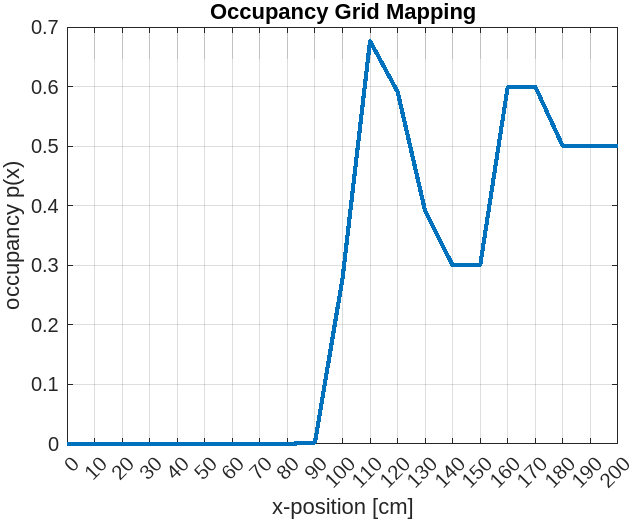
\includegraphics[width=0.5\textwidth]{Q2PMF.png} % Image path and size
            \caption{Probability Mass Function (PMF) of the occupancy grid map}
            \label{fig:image1} % Label for referencing the figure
        \end{figure}
    \end{solution}

    \question[25]
    In Problem 4 of the last homework assignment, you used EKF for landmark-based localization, where the line features in the environment played the role of landmarks. In this problem, you'll solve the same localization problem using particle filter, or in other words apply Monte Carlo Localization.

    \begin{solution}
    \end{solution}

    \question[(Bonus) 20]
    This \href{https://www.mathworks.com/help/nav/ug/landmark-slam-using-apriltag-markers.html}{linked Mathworks example} uses pose graph and factor graphs for SLAM, given odom-
    etry data and measurement data from April Tag markers being used as landmarks. You'll
    instead implement the EKF-SLAM algorithm on the same data, to obtain the locations of all
    landmarks and the trajectory of the robot.

    \begin{solution}
    \end{solution}
\end{questions}

\end{document}